\documentclass[paper,11pt]{geophysics}
%\documentclass[paper,twocolumn]{geophysics}
%\documentclass[manuscript]{geophysics}
%\documentclass[long]{geophysics}
% An example of defining macros


% An example of defining macros
\newcommand{\rs}[1]{\mathstrut\mbox{\scriptsize\rm #1}}
\newcommand{\rr}[1]{\mbox{\rm #1}}


\usepackage[english]{babel}
\usepackage[T1]{fontenc}
\usepackage[utf8]{inputenc}

\usepackage[hang,tableposition=top, labelfont=bf,textfont=it]{caption} % Custom captions under/above floats in tables or figures
\usepackage{threeparttable}

\usepackage{amsmath}


\usepackage{color}

%\usepackage{lineno}
%\linenumbers

\begin{document}
\begin{center}
\textbf{\LARGE
Characterizing the crustal architecture of the Parnaíba basin with passive-source seismology
}
\linebreak 

\textbf{Diogo Coelho$^{1*}$, Jordi Julià$^{1}$, Verónica Rodríguez Tribaldos$^{2}$ \& nicky White$^{2}$}
\linebreak 

\textit{
$^{1}$Departamento de Geofísica, Universidade Federal do Rio Grande do Norte, Capim Macio, Natal, CEP 59078-970, Brazil
\\
$^{2}$Bullard Laboratories, Department of Earth Sciences, University of Cambridge, Madingley Rise House, Madingley Road, Cambridge, CB3 0EZ, UK
\\
*Corresponding author (e-mail: locdiogo@gmail.com)
}

\end{center} 
\section{Abstract}

Lithospheric-scale processes, such as the origin and evolution of large cratonic basins, can create big footprints or signatures in the subsurface that can be observed by geophysical means. Our study area is the Parnaíba Basin and the main goal is to provide new images of the crust and lithosphere under the basin and highlight seismic discontinuities. A total of 9 broadband seismographic stations were installed within the PBAP project, along an approximately 500 km-long transect across the basin, with interstation spacing of around 50 km. We estimated crustal thickness and Vp/Vs ratio of the Parnaíba Basin by developing P-wave receiver functions. We also developed one-dimensional S-velocity models calculated from the joint inversion of P-wave receiver function and Rayleigh dispersion curves. Results from HK-Stacking, receiver function migration and joint inversion indicate that the Moho dips gently toward the depocenter of the basin (>42 km) and, in the eastern part, some mid-crust reflections at 15-20 km depth, indicating the presence of a mid-crust discontinuity bounding the Borborema Province. We have provided seismic evidence to discriminate the basement beneath of the Parnaíba basin into two blocks, Parnaíba and Teresina blocks, according to the S-velocity models and the cross-section of a migrated P-wave receiver functions across the basin.


\bigskip 
\textbf{Keywords:} Broadband Seismology, Parnaíba Basin, Crustal Architecture

%\bigskip 
%\textbf{Supplementary material:} [description of material] is available at https://doi.org/xxxx’. [GSL will assign the doi and url unless you already have one]

\bigskip 


The genesis and evolution of large intracratonic basins is an important geological issue that still not completely understood. The basin-forming mechanism and tectonical history of these basins has been much debated with no clear consensus emerging, because there are a varied mechanisms that leading to subsidence of the basin. The Parnaíba basin is one of three large Phanerozoic sedimentary basins in northern South America. This basin is surrounded by three	 larges cratonic areas, Amazonian, São Luís and São Francisco [\cite{de_almeida_brazilian_1981};\cite{de_brito_neves_neoproterozoic_2013};\cite{cordani_significance_2013}]. The Parnaíba basin is a large, sag-type cratonic basin with a saucer and roughly circular shape and its depocenter reaches up to 3.5 km thick [\cite{goes_feijo_1994}, \cite{vaz_bacia_2007} and \cite{daly_brasiliano_2014}].

Recently, \cite{fuck_rodinia_2008} show that the Precambrian basement of the Parnaíba Basin is composed of several crustal segments, which are the result of agglutination of the existing cratonic fragments (Amazonian, São Luís/West Africa and São Francisco/Congo). \cite{de_brito_neves_influence_1984} proposed the existence of a distinct but unexposed basement block beneath the center western part of the basin, trapped between the Amazonian craton and the Borborema orogenic belt, based in regional geology and isotope studies. Currently, \cite{de_castro_crustal_2014} and \cite{de_castro_geophysical_2016} used a large geophysical data set, involving airborne potential field, seismic and well log data, to reveal the basement inlier block. After this, the authors subdivided the Parnaíba Block into the Parnaíba and Teresina blocks. Follow the same ideia, \cite{daly_brasiliano_2014} described the Parnaíba Block with a large deep seismic profile and shed light on the important role of the two major igneous events in the basin development, with extensive extrusives in the Early Jurassic and widespread dykes and sills of Early Cretaceous age.

Knowledge of the crustal thickness is important for understanding the tectonic complexity of the basement. Thus, Moho relief of the South America was studied to several authors in the course of time, like \cite{feng_group_velocity_2004}, \cite{feng_upper_2007}, \cite{lloyd_moho_2010}, \cite{van_der_meijde_gravity_2013}, \cite{assumpcao_models_2013} and \cite{assumpcao_crustal_2013}. In this paper we characterize the crustal structure beneath the Parnaíba basin by mapping subsurface seismic discontinuities with teleseismic P-wave receiver functions, as proposed by \cite{langston_structure_1979}. The data set acquired in 9 seismographic stations, as showed in Figure \ref{mapa_estacoes_geologico} and Table \ref{tabela_estacoes}, is part of the Parnaíba Basin Analysis Project (PBAP), a collaboration among several universities and BP Energy do Brasil. We present estimates of the crustal thickness and Vp/Vs ratio at each station obtained through the H-$\kappa$ stacking procedure of \cite{zhu_moho_2000}, as well as S-velocity models obtained by joint inversion between observed receiver functions and surface-wave dispersion velocities from \cite{feng_upper_2007}, with the  inversion scheme of \cite{julia_joint_2000}. We used the common conversion point (CCP) technique, proposed by \cite{frassetto_improved_2010}, to produce a 2D cross-section for imaging seismic discontinuities beneath the basin.

Our results confirm previous findings of \cite{de_castro_crustal_2014} that the Parnaíba Basin basement are divided in Parnaíba and Teresina blocks. Results from H-$\kappa$ stacking, receiver function migration and joint inversion indicate the Moho dips gently toward the depocenter of the basin, displaying up to three different behaviors: A flat Moho in the depocenter of the basin, which showed the thickest crust (>42 km) and Vp/Vs ratio values arround 1,76; A thinning crust towards the eastern flank (<38 km), bounding with the Borborema Province, with Vp/Vs ratio of 1,73, which coincides with the low topographies; An almost flat Moho with thickness of 40 km and Vp/Vs ratio around 1,75 on the western border, bounding with the Araguaia Belt. We also noted a mid-crust reflections at 15-20 km depth, in the eastern part of the basin, indicating the presence of a mid-crust discontinuity. The mid-crust revels that the Teresina block is a part of the Borborema Province covered by the sediments of the Parnaíba basin and the Parnaíba block is a cratonic fragment, according to features displayed in the S-velocity model and in the cross-section of receiver function migration.

\begin{figure}[!ht]
\centering
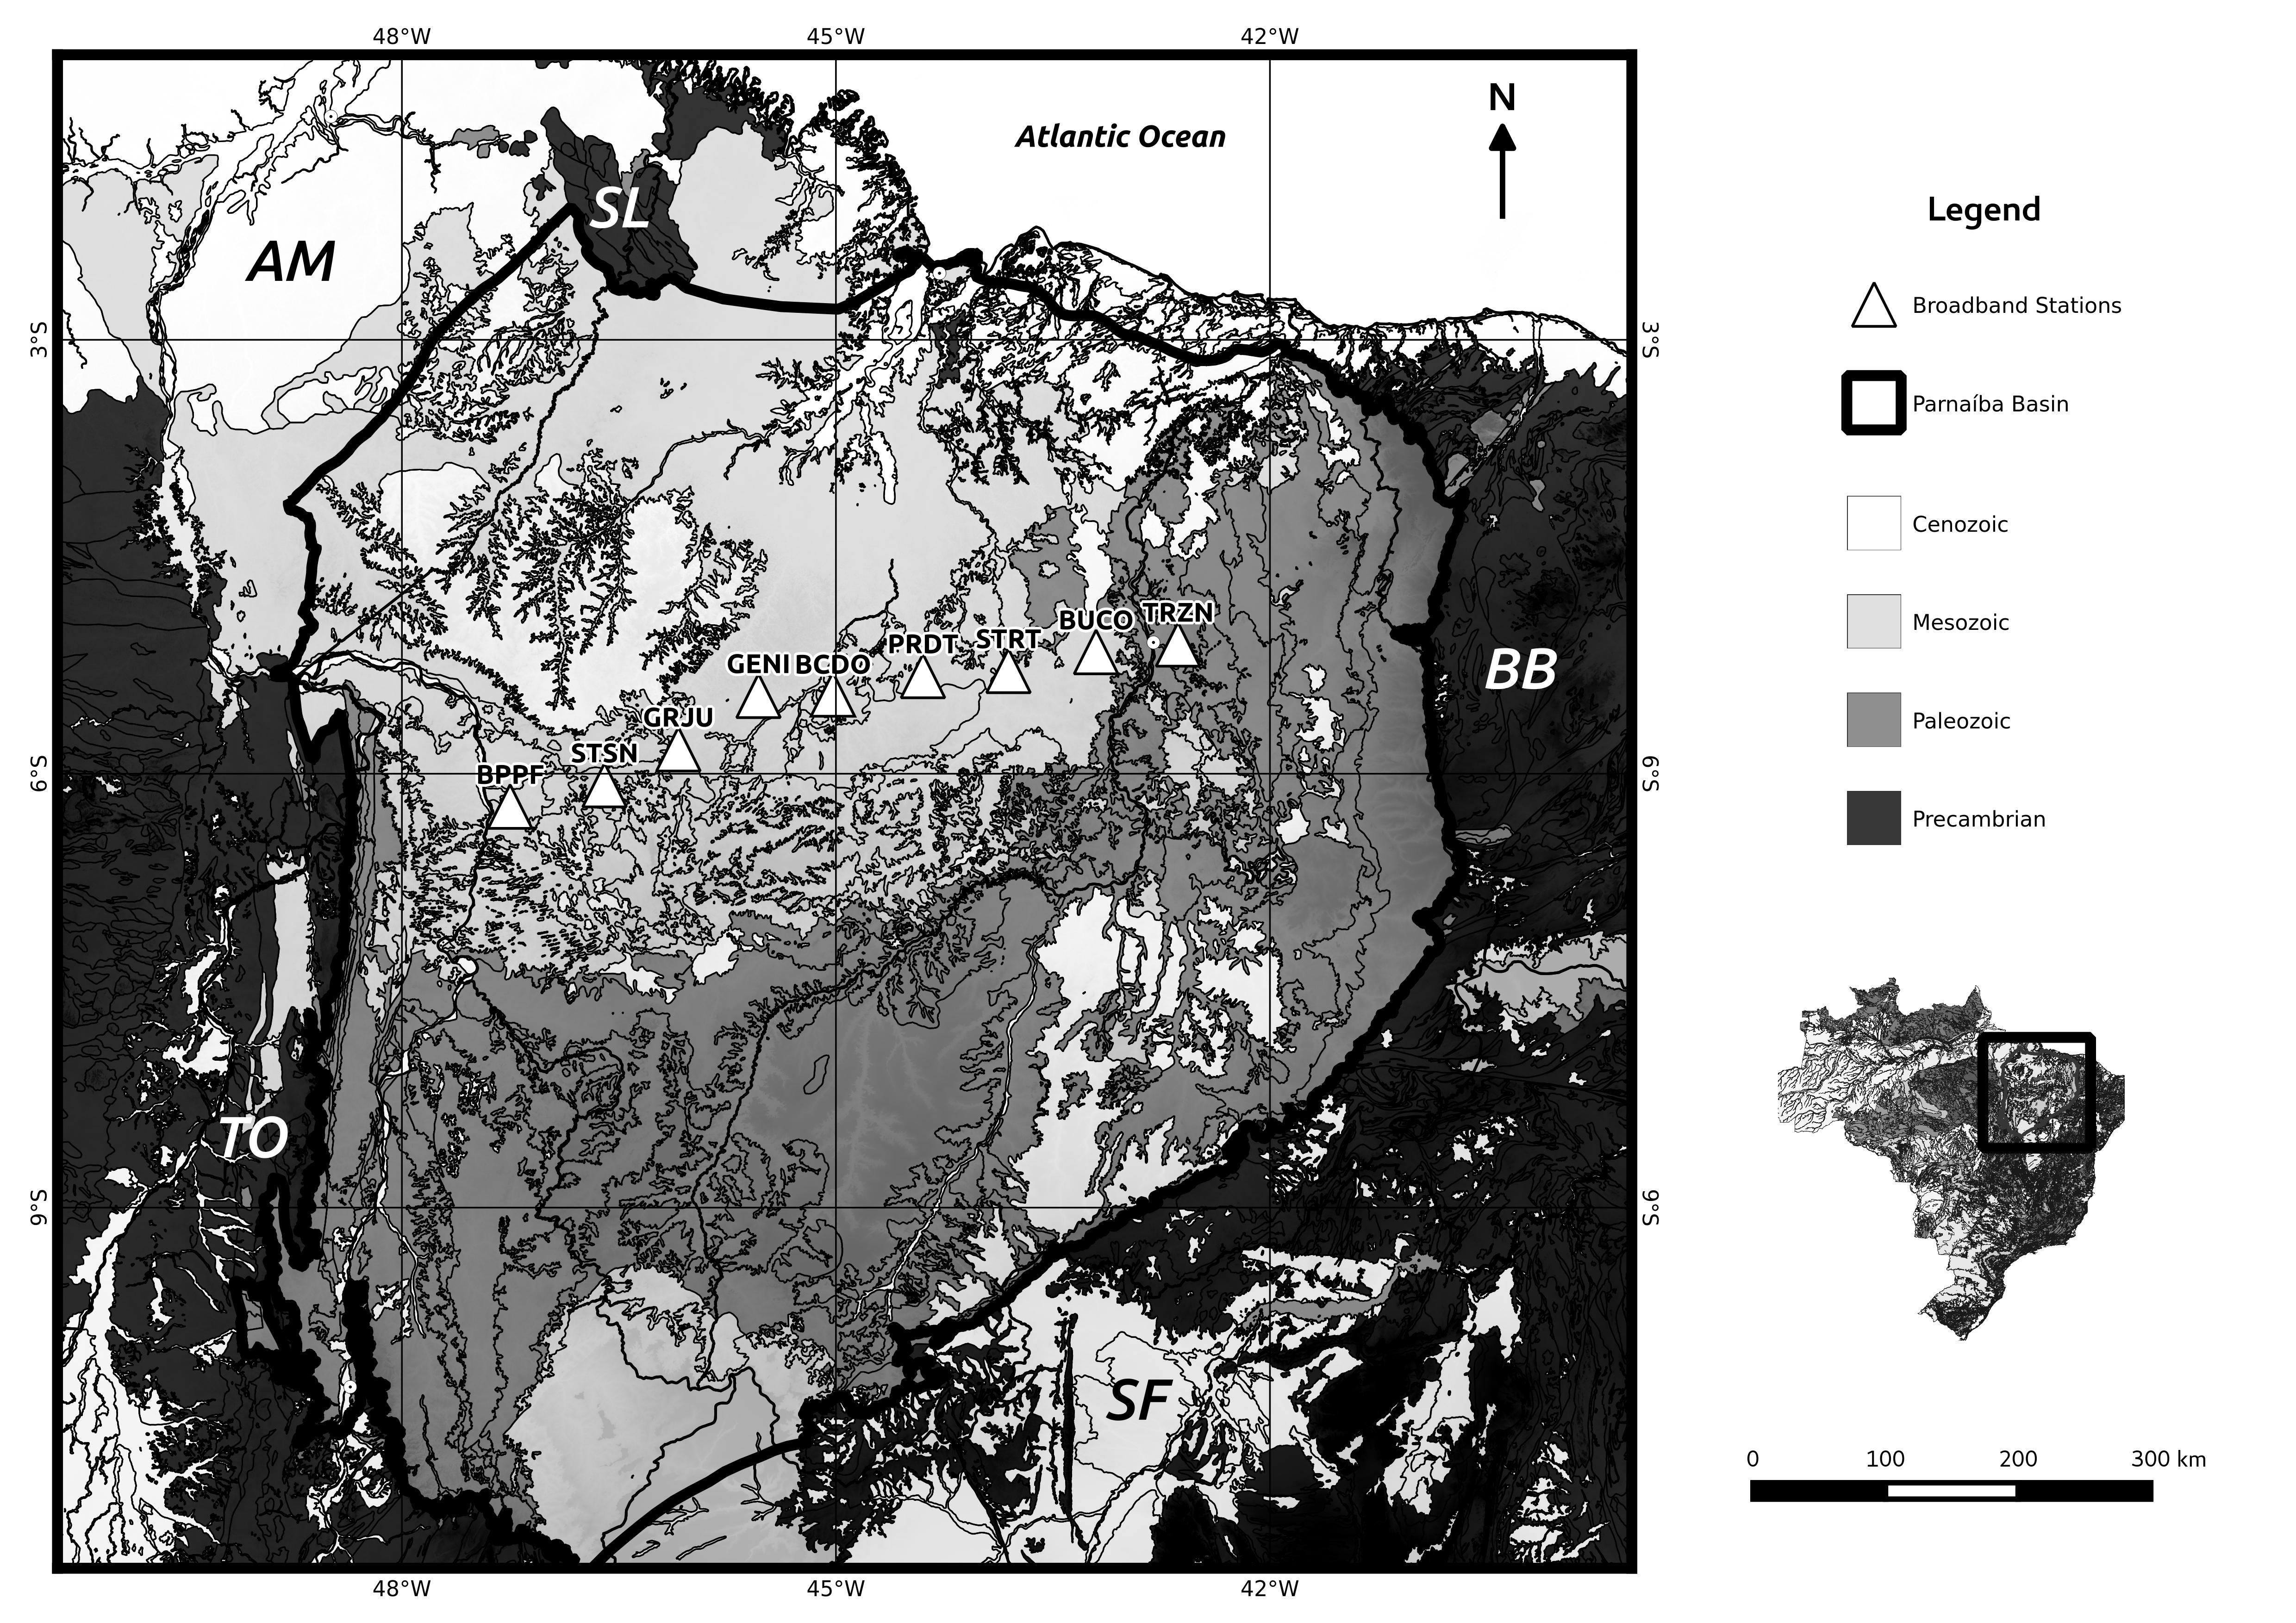
\includegraphics[width=0.9\textwidth]{Fig/Mapa_geologico_BP_grey.jpg}
\caption{Geological Map with the location of PBAP project stations. AM - Amazonian Craton, BB - Borborema Province, SF - São Francisco Craton, SL - São Luís Craton, TO - Tocantins Province.}
\label{mapa_estacoes_geologico}
\end{figure}

\section{Geological Background}

\cite{de_castro_geophysical_2016} call attention to shear zones as probable main protagonist in the evolution of the Parnaíba basin. This basin is encircled by sutures zones associated with cratonic blocks collisions, as presented by \cite{daly_brasiliano_2014}, \cite{de_castro_crustal_2014} and \cite{de_castro_geophysical_2016}, as shown in the Figure \ref{mapa_estacoes_geologico}. On the eastern side of the basin, the Araguaia suture zone represents the final Neoproterozoic collision between the Amazonian craton and the pre-Neoproterozoic Parnaíba block [\cite{fuck_rodinia_2008}, \cite{brito_neves_basement_2014}]. On the eastern side of the basin, the Transbrasiliano Lineament, a continental-scale discontinuity characterized by strong magnetic anomalies and by low S wave velocities in the mantle [\cite{fairhead_champ_2003}; \cite{feng_group_velocity_2004};  \cite{brito_neves_basement_2014}], controls the internal rift geometry and form a 150 km wide rift zone. On the septentrional boundary, the Gurupi Belt represents the deformation zone between the Parnaíba block and São Luís craton. This belt is a sequence of Paleoproterozoic rock assemblages reworked in the Neoproterozoic during a Brasiliano phase \citep{klein_gurupi_2005}. These lineaments also form Precambrian lithospheric-scale boundaries that were identified in a deep crustal seismic reflection profile across the Parnaíba basin \cite{daly_brasiliano_2014} and represent the collisional sutures of the Amazonian and the São Francisco cratons \cite{de_castro_crustal_2014}.

The basement beneath the Parnaíba basin was subdivided into 2 crustal blocks, Parnaíba and Teresina, by \cite{de_castro_geophysical_2016}, in accordance with their magnetic and gravity signatures. The Teresina block shows a high-amplitude reflexion called by \cite{daly_brasiliano_2014} as mid-crustal reflectivity (MCR). This discontinuity is defined as a subhorizontal, curved feature up to 3 km thick terminate into the acoustically featureless Parnaíba block. \cite{daly_brasiliano_2014} show that below this mid-crustal zone are a series of subhorizontal, moderate amplitude events, the base of which appears to define a Moho locally at about 38 km depth. This value supports results found by \cite{de_castro_crustal_2014} and \cite{de_castro_geophysical_2016}. As said by \cite{fuck_rodinia_2008}, \cite{de_castro_crustal_2014} and \cite{de_castro_geophysical_2016}, the Parnaíba Block represents an old continental fragment over a relatively thickened crust, around 42 km, in relation to surrounding crustal zones and its existence has been proposed on the basis of geophysical evidence in addition to petrography and geochronology of the basement rocks. 

The evolution of the Parnaíba basin involved five primary tectono-sedimentary sequences and two magmatic pulses. The present-day sag basin consists of at least four tectono-sedimentary sequences separated by regional unconformities, comprising a distinct deposition history [\cite{goes_feijo_1994}, \cite{vaz_bacia_2007}]. The basin has an asymmetric geometry, as can be seen in \cite{daly_brasiliano_2014}, a elevated western margin and an eastern margin dipping gently. According to \cite{goes_feijo_1994} the Parnaíba basin depositional history spans the early Paleozoic to the Mesozoic, as seen in \ref{mapa_estacoes_geologico}. The basin is composed of thick, primarily siliciclastic, epicontinental sequences, not to mention Cenozoic alluvial and aeolian deposits.

\section{Methodology}

Teleseismic body waveforms recorded at a three-component seismic station contain information on the earthquake source, the earth structure in the vicinity of both source and the receiver, and mantle propagation effects [\cite{langston_structure_1979} ,\cite{ammon_isolation_1991}, \cite{cassidy_numerical_1992}, \cite{ligorria_iterative_1999}]. The receiver function is obtained by removing the effects of source and mantle path by way of the deconvolution of the vertical components from the corresponding horizontal components, therefore isolating the earth structure neighbouring the receiver \citep{ligorria_iterative_1999}. The incident P wave energy from teleseismic events will be converted to S wave (Ps) after the interaction with subsurface discontinuities and arrive at the station within the P wave coda after the direct P wave. The analysis of the amplitudes and traveltimes of the interaction phases provides important constraints on the seismic structure under the station \citep{zhu_moho_2000}.

We have selected teleseismic P-waveforms recorded by the PBAP project stations shown in Figure \ref{mapa_estacoes_geologico}. These stations have sources with epicentral distance raging between 30 and 90 and body wave magnitudes above 5.5 mb. Our dataset is composed by 8  stations using three-component Meridian Compact Posthole sensor and one station using three-component Guralp sensor. The stations coordinates and recording times for the PBAP project considered in this study are listed in Table \ref{tabela_estacoes}. To compute the receiver functions, both radial and transverse, we applied the same methodology of \cite{julia_deep_2008} and \cite{luz_bulk_2015}, utilising a Gaussian filters of the 2.5.

\begin{table}[! htpb]
\centering
	\small
	\begin{threeparttable}
	\caption{Station coordinates and recording time window from Parnaíba basin.}
	\begin{tabular}{c c c c}
    \hline
    Station & Latitude & Longitude & Recording time \\ \hline
    BPPF & -6.2271 & -47.2518 & 2016.188 – 2016.345 \\
	BUCO & -5.1586 & -43.2010 & 2016.118 – 2016.344 \\
	GENI & -5.4612 & -45.5344 & 2016.105 – 2016.346 \\
	GRJU & -5.8308 & -46.0882 & 2016.104 – 2016.345 \\
	PRDT & -5.3241 & -44.3974 & 2016.106 – 2016.344 \\
	STSN & -6.0787 & -46.5986 & 2016.105 – 2016.345 \\
	STSR & -5.2889 & -43.8063 & 2016.119 – 2016.344 \\
	TRSN & -5.1056 & -42.6344 & 2016.118 – 2016.344 \\
	BCDO & -5.4517 & -45.0203 & 2015.222 – 2016.293 \\ \hline
    \end{tabular}
    \label{tabela_estacoes}
	\end{threeparttable}
\end{table}

To estimate the crustal thickness and Vp/Vs ratio from the receiver functions we utilise the H-$\kappa$ stacking technique of \cite{zhu_moho_2000}. This procedure performs a grid-search  over a stacking surface built by summing a weighted combination of the Ps, PpPs and PpSs+PsPs amplitudes. In this procedure, the P-wave velocity for the layer, average of 6.3 km/s to the basin, and the phase weights must be specified a priori, as shown in Table \ref{tabela_hk_stacking}. Confidence  bounds for the thickness and Vp/Vs estimates have been obtained by bootstrapping, as explained in  \cite{efron_statistical_1991}, the receiver function waveforms at each station with 200 replications. \cite{luz_bulk_2015} have a detailed explain about this procedure.

S-wave velocity models beneath PBAP stations in the Parnaíba basin have been obtained through the inversion scheme of \cite{julia_joint_2000}. To ensure that both data sets sample similar regions of the Earth, we identified the surface-wave tomographic cell enclosing each station in our study and extracted the local group velocity curve for the tomographic cell. We then inverted the receiver functions jointly with the extracted dispersion curve, in this case, dispersion curves from \cite{feng_upper_2007}. The data sets were normalized for the different number of data points and physical units prior to inversion. The procedure includes an influence factor equal to 0.5 that weights the contribution of each data and to provide a good compromise between fitting the receiver functions and the dispersion velocities. The starting model for the linearized procedure is the 1D velocity model measured by \cite{almeida_crustal_2015}. Some instabilities that drive the iterative process away from convergence was overcome through smoothness constraints in the velocity profiles, at the expense of losing resolution in the inverted models. Usually, a total of 9 iterations sufficed for the inversion process to converge to a final S-velocity model.

The final step in our analysis was the migration and stacking of P-wave receiver functions for the PBAP project seismic. We followed the same approach as in \cite{almeida_crustal_2015}, which one investigated the crustal architecture across the
Borborema Province. In total, our expanded dataset includes 744 receiver function waveforms throughout the basin. To stack the receiver function waveforms we utilized the common conversion point (CCP) migration and stacking procedure of \cite{frassetto_improved_2010}. The procedure combines the CCP stacking of \cite{gilbert_images_2004} with the phase-weighting scheme of \cite{schimmel_noise_1997} to enhance coherent P-to-S conversions in the stacks. A detailed explain about this
procedure can be found in \cite{frasseto_receiver_2013} and \cite{almeida_crustal_2015}.

\section{Results}

\begin{figure}[!ht]
\centering
\includegraphics[width=0.8\textwidth]{Fig/mosaico_GRJU_TRSN.png}
\caption{Moisaic showing H-$\kappa$ stacking results for GRJU (top) and TRSN (bottom) stations. For each station the top panels display the receiver function, radial (black lines) and tranverse (red lines), sorted by backazimuth and the map with the location of the earthquakes utilised (yellow stars). The bottom panels display the receiver function stacked with the Ps, PpPs, and PpSs+PsPs phases times superimposed to the receiver functions and a figure showing the H-$\kappa$ stacking screen.}
\label{moisaic_FR}
\end{figure}

Analising the results displayed in the Figure \ref{moisaic_FR}, we can see the radial and transverse receiver functions selected for the GRJU and TRSN stations. A simple inspection of the waveforms reveals important properties of the propagating medium beneath each station. Comparing the amplitude of the transverse (red lines) and radial (black lines) receiver functions for both stations, we observe that the transverse receiver functions generally display small amplitudes compared to the corresponding radial waveforms. For a laterally homogeneous media is expected a transverse receiver function have an amplitude equal to zero. In the Figure \ref{moisaic_FR} we see small transverse amplitudes indicating that the medium under the GRJU station can be approximate as laterally homogeneous and isotropic. Moreover, in the TRSN station the amplitude of the tranverse component is higher than the GRJU station, thus the medium beneath this station is different of the GRJU station, and we need some precaution in our estimate. Also, we can identify the signature of the sedimentary cover, negative peak, in all the radial waveforms in both stations. The shift in the main peak, for instance, is due to a large Ps phase generated at the sediment – bedrock interface that arrives shortly after the incoming P-wave, and cannot be resolved by the Gaussian filter \citep{cassidy_numerical_1992}. Also other apparent peaks and troughs between 1 and 3 s are also caused by the interaction of the impinging P-wavefront with sedimentary structure. Finally, the Ps phase generated at the Moho is generally apparent in all the waveforms at about 5 s, but the multiply reverberated phases in the bulk crustal structure are generally harder to identify. The wavelengths of the reverberated phases are shorter than those of the Ps phase, and a gradational crust–mantle boundary could
reduce their amplitudes significantly \citep{julia_joint_2000}. Some multiples are hard to detect in the waveforms, especially the PpSs+PsPs phase, Figure \ref{moisaic_FR}, and this variability is translated into large confidence bounds during the bootstrap resampling \citep{julia_deep_2008}. We can see a backazimuth dependence of the receiver function in the top panel of the Figure \ref{moisaic_FR}, but this problem is not a problem because our earthquakes have a restrict backazimuth window. 

\begin{table}[! htpb]
\centering
	\small
	\begin{threeparttable}
	\caption{H-$\kappa$ stacking parameters and results from Parnaíba basin.}
	\begin{tabular}{c c c c c c c c c}
    \hline
    Station & n & Vp & w1 & w2 & w3 & h0 & H(km) & Vp/Vs \\ \hline		
    BPPF & 5 & 6.3 & 0.4 & 0.4 & 0.2 & 41 & $41.20 \pm3.857$ & $1.750 \pm  0.075$ \\
	BUCO & 11 & 6.3 & 0.4 & 0.3 & 0.3 & 40 & $38.00 \pm 1.33$ & $1.735 \pm 0.033$ \\
	GENI & 7 & 6.3 & 0.4 & 0.3 & 0.3 & 44 & $44.00 \pm 2.05$ & $1.766 \pm 0.088$ \\
	GRJU & 11 & 6.3 & 0.4 & 0.3 & 0.3 & 40 & $41.00 \pm 1.41$ & $1.827\pm 0.047$ \\
	PRDT & 11 & 6.3 & 0.4 & 0.3 & 0.3 & 40 & $38.70 \pm 3.36$ & $1.815 \pm 0.081$ \\
	STSN & 12 & 6.3 & 0.4 & 0.3 & 0.3 & 40 & $40.50 \pm 1.56$ & $1.751 \pm 0.043$ \\
	STSR & 8 & 6.3 & 0.4 & 0.3 & 0.3 & 40 & $38.59 \pm 0.23$ & $1.693 \pm 0.011$ \\
	TRSN & 12 & 6.3 & 0.4 & 0.3 & 0.3 & 40 & $38.00 \pm 2.26$ & $1.751 \pm 0.052$ \\
	BCDO & 3 & 6.3 & 0.4 & 0.3 & 0.3 & 40 & $40.00 \pm 3.34$ & $1.700 \pm 0.081$ \\ \hline
    \end{tabular}
	\begin{tablenotes}\footnotesize
	\item[*] The table includes the number of waveforms (n), P-wave velocity assumed (Vp), weights for the Ps (w1), PpPs (w2), and PpSs + PsPs (w3) phases.
    \end{tablenotes}
    \label{tabela_hk_stacking}
	\end{threeparttable}
\end{table}

Table \ref{tabela_hk_stacking} lists the H-$\kappa$ stacking results for the PBAP stations in the Parnaíba basin. The crustal thicknesses range between 38 and 44 km and are generally constrained within 3 km. Overall, these values are in excellent agreement with the estimates from previous continental scale studies, as \cite{feng_upper_2007}, \cite{lloyd_moho_2010} and \cite{assumpcao_crustal_2013}. Results from HK-Stacking, receiver function migration and joint inversion indicate the Moho dips gently toward the depocenter of the basin, nearby the GRJU station, displaying up to three different behaviors: A flat Moho in the depocenter of the basin, which showed the thickest crust. A thinning crust towards the eastern flank, bounding with the Borborema Province, as can be observed in the S-velocity models in the Figure \ref{moisaic_joint_inversion} and in the ccp migration cross-section in the bottom of the Figure \ref{moisaic_migration}. We can see a consonance among the crustal thickness nearby the Borborema Province calculeted by our data and by the studies of \cite{pavao_upper_lower_2013}, \cite{almeida_crustal_2015} and \cite{luz_bulk_2015}. We have a lack of works in seismology in the western part, but we can find some analogous results in \cite{de_castro_crustal_2014} and \cite{daly_brasiliano_2014}, notwithstanding our estimates recover a thickest crust comparing with these authors.

Studying the variation of Vp/Vs ratio on grounds of the complexity of the crust composition should provide important constraints of the geological history. Although, the Vp/Vs values are more variable and less tightly constrained \citep{julia_deep_2008}. Comparing the Vp/Vs ratio of the Table \ref{tabela_hk_stacking}, we can see that the bulk composition of the eastern part of the basin, close-by 1.73, is more felsic compared to  western part, around 1.76, according to \cite{christensen_poissons_1996} classification. \cite{chevrot_australia_2000} mention that the Vp/Vs ratio varies as a function of crustal thickness inside a geological province. Table \ref{tabela_hk_stacking} indicates an increment of Vp/Vs ratio with increasing crustal thickness, as well as in the bottom panel of the Figure \ref{moisaic_migration}. GRJU station shows a Vp/Vs of $1.827\pm 0.047$, this can be explained due to the increase of the thickness, concomitantly growth the mafic lower crust (granulite composition), thus, according to \cite{christensen_poissons_1996}, is expected high values of Vp/Vs, as we can check in the stations in the western part of the basin. Similarly, \cite{christensen_poissons_1996} and \cite{julia_deep_2008} suggest that high values can be related with a mafic crust or a concentration of basaltic rocks, correlating with gross thickness of diabase intrusions in the center of the basin \citep{daly_brasiliano_2014}, as observed in the Vp/Vs ratio for the PRDT station.

\begin{figure}[!ht]
\centering
\includegraphics[width=1\textwidth]{Fig/comparacao_joint_inversion.png}
\caption{Joint inversion models for each station sorted according the station location in the Figure \ref{mapa_estacoes_geologico}. The top panel displays the S-velocity models and in the bottom panel the interpretation of the S-velocity models.}
\label{moisaic_joint_inversion}
\end{figure}

Joint inversion models in the Figure \ref{moisaic_joint_inversion} reveal two different structural patterns according to our interpretation, shown in the lower panel.  First of all, we can differentiate in the top of each model a sedimentary layer, characterized by low velocities (blue color). We do not insert a priori information about a sedimentary layer in the start model, as seen in the start model of \cite{almeida_crustal_2015}, thus the inversion been able to recover the sedimentary structure correctly, mainly the thickness of the basin (> 4km). The analyzed stations data in the Teresina Block (PRDT, STRT, BUCO and TRSN) allow us to interpret a mid-crust discontinuity depth between 15 km and 25 km. This discontinuity is indicated by a high velocity layer (red color), but we cannot identify this discontinuity in the western part, as shown by \cite{daly_brasiliano_2014}. The mid-crust discontinuity is called by \cite{pavao_upper_lower_2013} as upper-lower crust discontinuity, latterly interpreted as detachment zone by \cite{almeida_crustal_2015}. Teresina Block shows a crustal compartimentation, with a Moho discontinuity well-identified (sharp discontinuity), however, Parnáiba Block exhibits a diffuse Moho, probably a gradational boundary. In the Parnáiba Block is not observed a mid-crust discontinuity, or a cleary segmentation of the crust, as can be observed in the Figure \ref{moisaic_joint_inversion}. The thicknesses from the inverted models, as expected, are in good agreement with the thicknesses calculeted from H-$\kappa$ stacking, Table \ref{tabela_hk_stacking}. The high velocity nearby to 5 km of depth can be related with some basaltic intrusions ou mafic bodies, or is just an artefact created due to lack of a priori information about the sedimentary layer.

\begin{figure}[!ht]
\centering
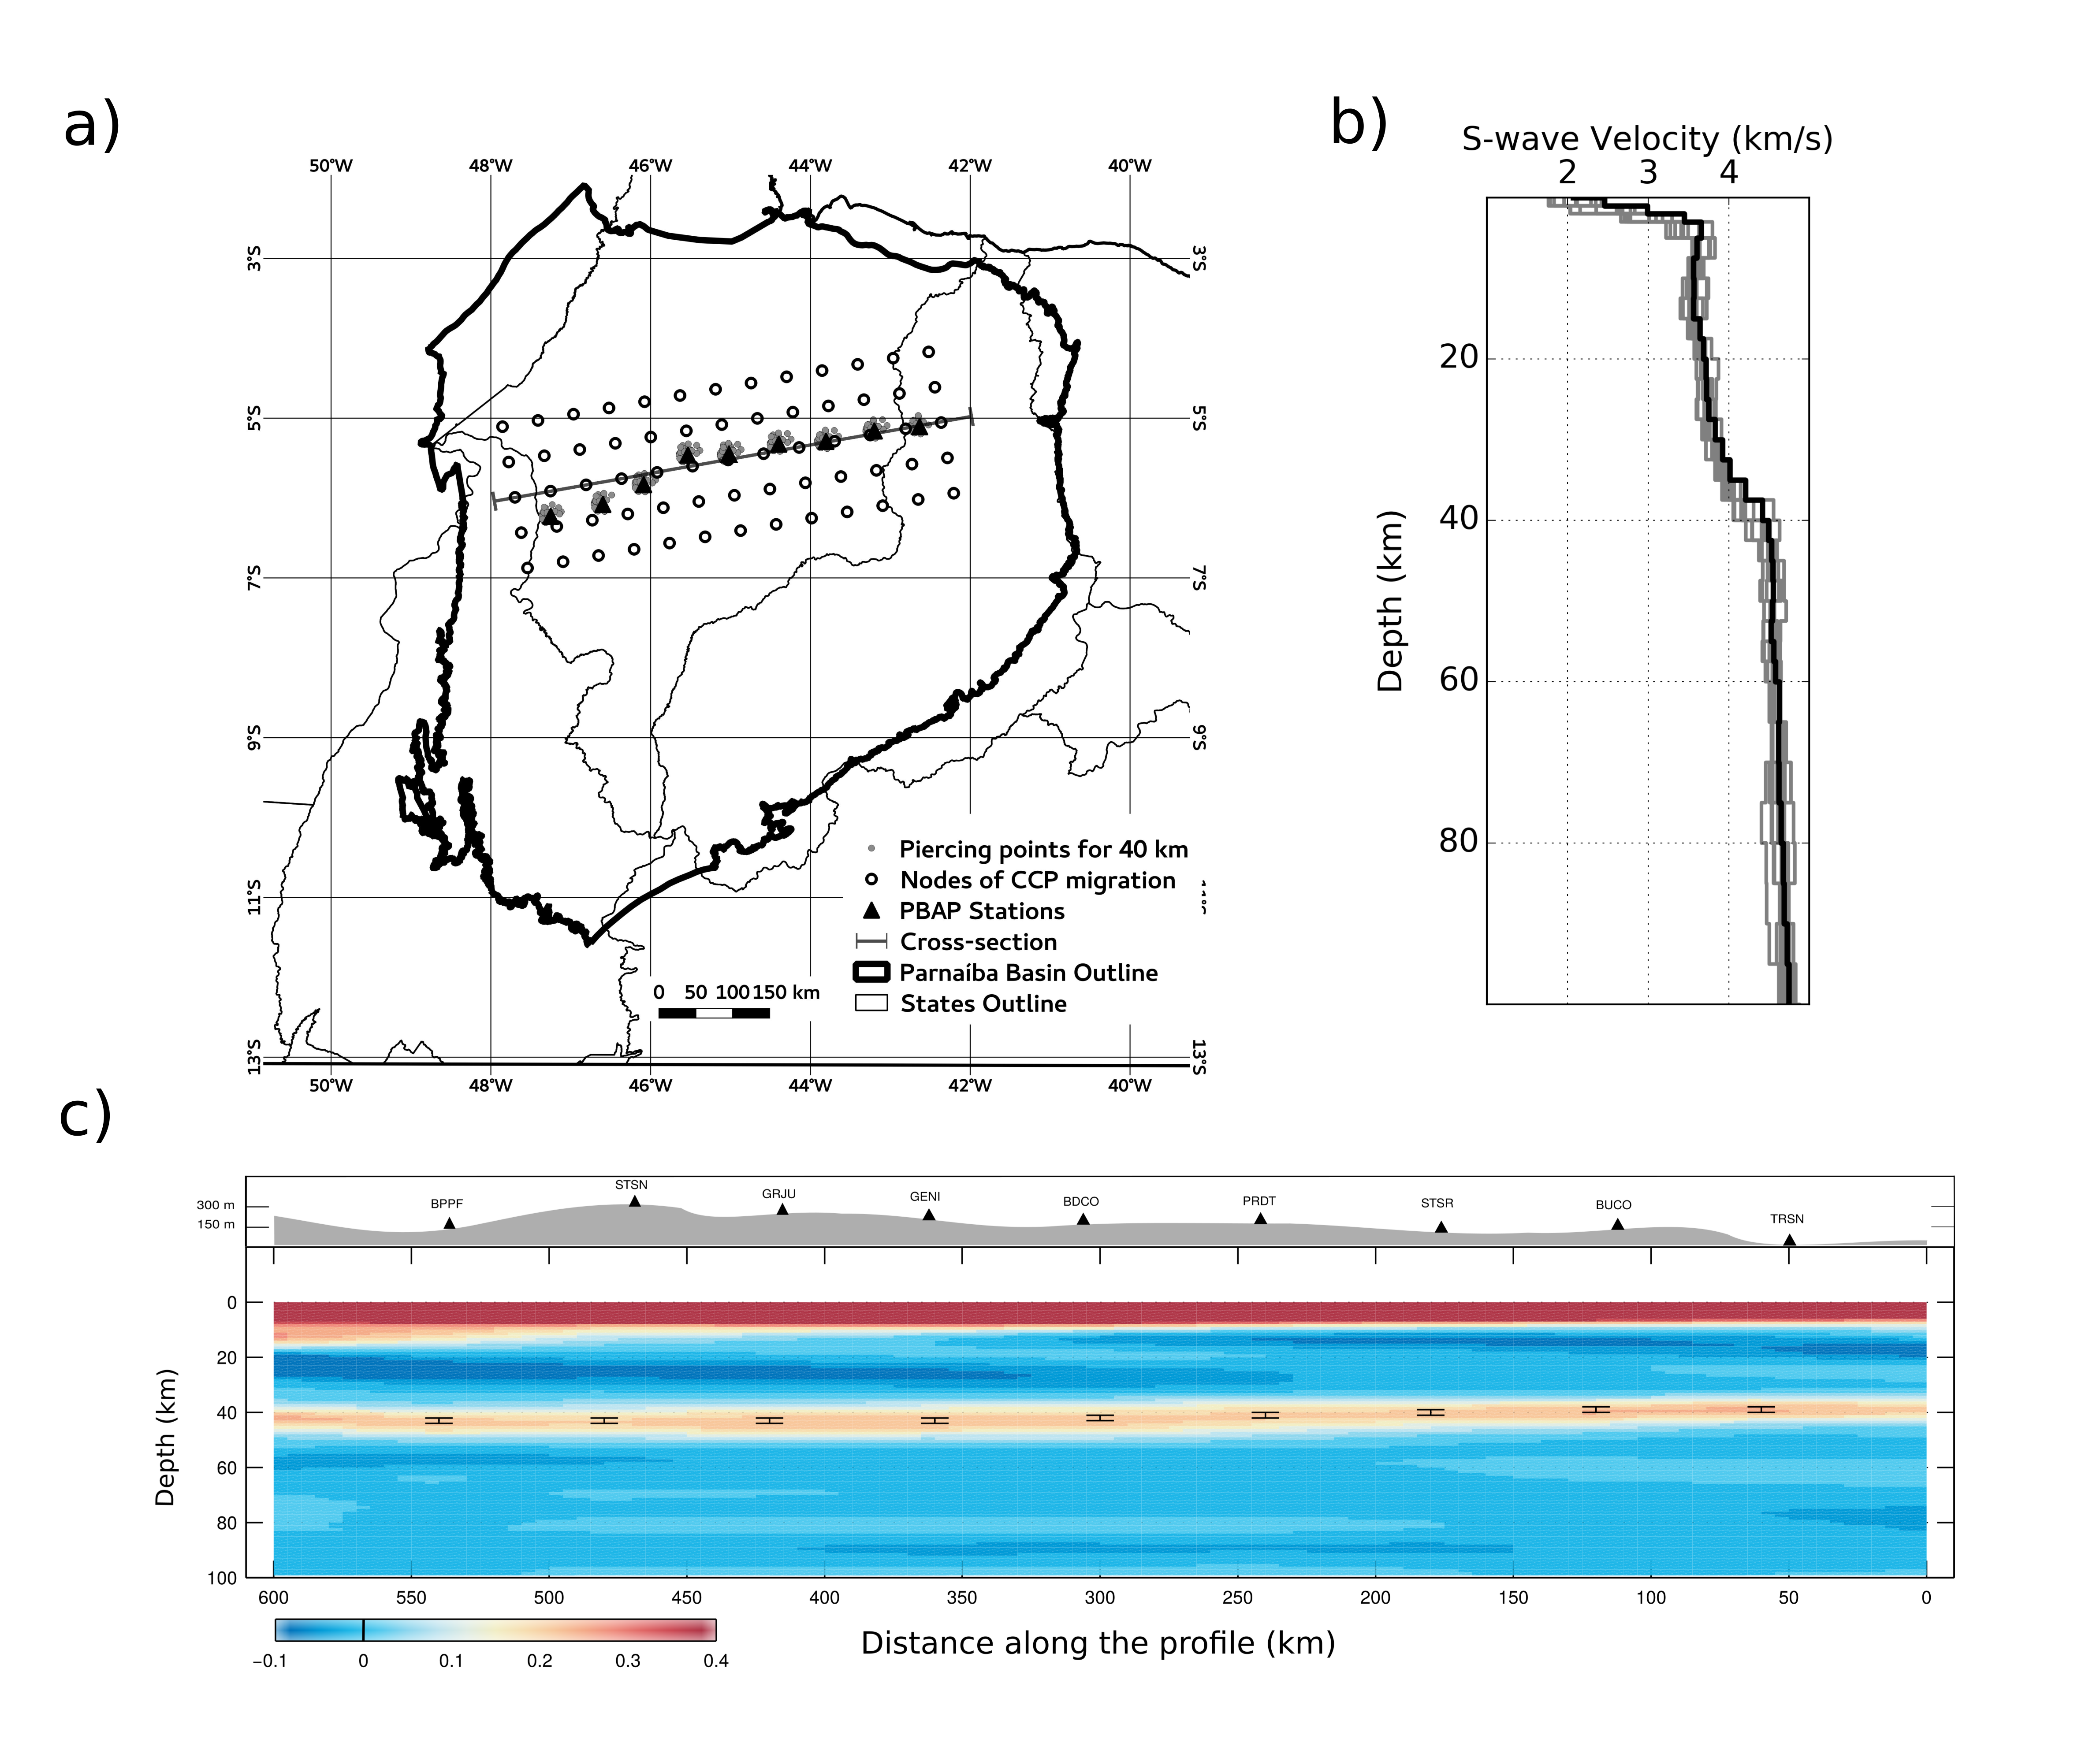
\includegraphics[width=1\textwidth]{Fig/section_migration.png}
\caption{Moisaic and H-$\kappa$ stacking results for TRSN station. The top panels display The receiver function waveforms selected sorted by backazimuth for TRSN station and the location of the earthquakes analised. The bottom panels display the receiver function stacked with the Ps, PpPs, and PpSs+PsPs phases times superimposed to the receiver functions and H-$\kappa$ stacking surface}
\label{moisaic_migration}
\end{figure}

The migrated cross-section, Figure \ref{moisaic_migration}, obtained through the receiver function CCP stacks indicates that the crustal basement of the Parnaíba Basin can be divided into two blocks, equivalently to the S-velocity model results. The separation between the western and eastern side is evident, due to the structural pattern of each block. The major discontinuities detected in the cross-section is at 15–25 km and at 38–44 km depth, mid-crustal and Moho discontinuity, respectively. Both discontinuities present a gently slope, but they dips in opposite directions, as seen in the lower panel of the Figure \ref{moisaic_migration}. Moho dips gently toward the depocenter of the basin, meanwhile the mid-crust discontinuity dips toward the Borborema Province. Published results of crustal structure for the Parnaíba Basin, \cite{de_castro_crustal_2014} and \cite{daly_brasiliano_2014}, identify a deeper crust–mantle boundary, as well as our H-$\kappa$ stacking and Joint Inversion results. \cite{daly_brasiliano_2014} recognise the shallower anastomosing discontinuity, but just locally. \cite{de_castro_crustal_2014} create a interpretative model for airborne gravity and magnetic data of the Parnaíba Basin, and divided the basement into upper, middle and lower crust segments. Another interesting relation can be observed within the Parnaíba Basin, the Figure \ref{moisaic_migration} reveals that the eastern side, regions of low topography, is characterized by a thin crust (38 km), while regions of elevated topography, current depocenter, tend to display a crust of 41 km or thicker. This behavior is controversial, because is intuitive that the current depocenter needs to be the lowest part of the basin. Additionally, \cite{almeida_crustal_2015} report the same behavior within the Borborema Province.

\section{Tectonic implications}

The most important finding in our study is the capability to divide the Parnaíba Basin basement into two blocks using passive-source seismology, following the statement propused by \cite{de_castro_crustal_2014}. The presence of an intra-crustal discontinuity at about 10–25 km depth within the Teresina Block can be related with a buried part of the Borborema Province covered by sediments of the Parnaíba Basin, because both \cite{pavao_upper_lower_2013} and \cite{almeida_crustal_2015} reported this same discontinuity in the Borborema Province. \cite{almeida_crustal_2015} interpreted this discontinuity as a detachment zone that resulted from Mesozoic extension, and proposed that it might be connected with a widespread network of shear-zones, which would in turn have helped accommodate extension within the brittle upper crust. But, to confirm this statement we need stations covering regions along the Brasiliano Lineament, because if this lineament affect this reflection pattern, this structures are older than Mesozoic age. 

Previosly, \cite{daly_brasiliano_2014} reported the Parnaíba block as a "seismically transparent block", but, fortunately, we could calculate Moho thickness with a good precision. Moreover, we cannot identy some internal strutures in this block. We interpreted, as well as \cite{fuck_rodinia_2008}, \cite{brito_neves_basement_2014} and \cite{assumpcao_crustal_2013}, that the Parnaíba Block is an old cratonic fragment. Analising the internal structure of Parnaíba block through of receiver functions is hard because the velocity contrast is not so high and some mineral phase changes are transitional, as we can see in the work of \cite{assumpcao_shield_2002}. Thus, we are not be able to iluminate the internal structure.

\section{Conclusions}

We have provided seismic evidence of the subdivision of the block beneath of the Parnaíba basin. Our results are consistent with the interpretation of \cite{de_castro_crustal_2014}, which postulated that the Parnaíba Basin basement are divided in Parnaíba and Teresina blocks according the S-velocity models and cross-section of a migrated P-wave receiver functions. Summarizing, we have obtained 9 point estimates of crustal thickness and bulk Vp/Vs ratio across the Parnaíba basin of NE Brazil. S-velocity models and cross-section of a migrated P-wave receiver functions in the Parnaíba Basin have demonstrated the existence of two main seismic discontinuities characterizing the crustal architecture of the basin. The deeper discontinuity displays values ranging between 38 and 44 km, and has been identified with the crust–mantle boundary; the shallower discontinuity occurs at depths of 15–25 km and preferentially within western part of the basin, region of thin crust, which coincides with the low topographies.

\bibliographystyle{seg.bst}
\bibliography{References.bib}
    
\end{document}
